오늘 A 학교에서 $1$번부터 $N$번까지 번호가 매겨진 $N$명의 학생이 $100$미터 달리기 경주를 하려고 합니다.

이때 여러분은 다음과 같은 정보를 총 $M$개 알고 있습니다.

\begin{itemize}
\item $i$ $j$: $i$번 학생과 $j$번 학생이 달리기 경주를 할 경우, 항상 $i$번 학생이 결승선에 먼저 들어옵니다.
\end{itemize}

단, 여러분의 정보는 언제나 정확하기 때문에, 모순되는 정보는 주어지지 않습니다. 또한, 어떤 두 학생을 골라도 기록이 서로 같지 않습니다.

여러분은 이 $N$명의 학생이 달리기 경주를 했을 때 결승선에 가장 먼저 들어온 $K$명에게 상을 주려고 합니다. 그러던 중 여러분은 다음과 같은 고민에 빠졌습니다.

\begin{itemize}
\item 학생들의 기록이 어떻게 결정되어도 가장 먼저 들어온 $K$명의 집합이 항상 동일하다면, 달리기 경주가 재미없게 됩니다.
\end{itemize}

예를 들어, $4$명의 학생이 있고 그 관계가 다음과 같다고 생각합시다. $i$에서 $j$로 향하는 화살표는 $i$번 학생이 항상 $j$번 학생보다 먼저 들어옴을 의미합니다.

\begin{center}
  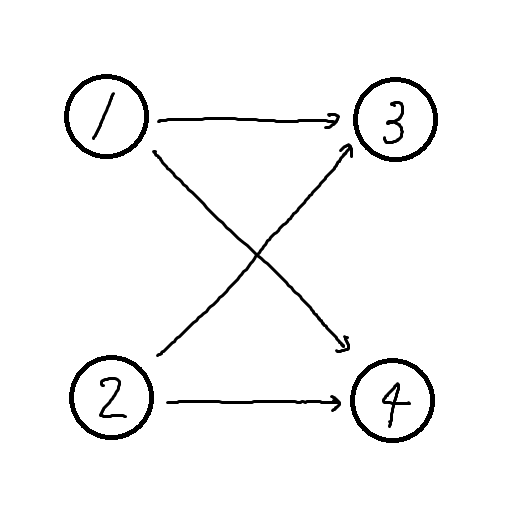
\includegraphics[scale=0.5]{winnerset.png}
\end{center}

이때 $K=2$라면 가장 먼저 들어온 $2$명은 항상 $1$번 학생과 $2$번 학생이므로 달리기 경주가 재미없게 됩니다.

$K=1,2,\ldots,N$에 대해 각각, $K$명에게 상을 줄 때 달리기 경주가 재미없게 되는지 구하는 프로그램을 작성해 주세요.